\chapter{Конструкторская часть}

В данном разделе выделяются требования к программному обеспечению, приводятся схемы алгоритмов, описываются используемые типы и структуры данных, и показывается структура программного обеспечения.

\section{Требования к программному \newline обеспечению}

Программное обеспечение должно обеспечить работу следующих функций:

\begin{itemize}
	\item загрузка модели предмета;
	\item изменение скорости предмета в интерактивном режиме;
	\item вращение, перемещение и масштабирование модели.
\end{itemize}

Требования, которые предъявляются к программе:

\begin{itemize}
	\item время отклика программы должно быть менее 1 секунды для корректной работы в интерактивном режиме;
	\item программа должна корректно реагировать на любые действия пользователя.
\end{itemize}

\section{Разработка алгоритмов}

На рисунке \ref{img:move-object} представлена схема алгоритма образования волновой поверхности, на рисунке \ref{img:draw-water} --- её отрисовка. На рисунке \ref{img:move-object} показана схема алгоритма перемещения предмета, на рисунке \ref{img:draw-object} --- его отрисовка.

\begin{figure}[H]
	\begin{center}
		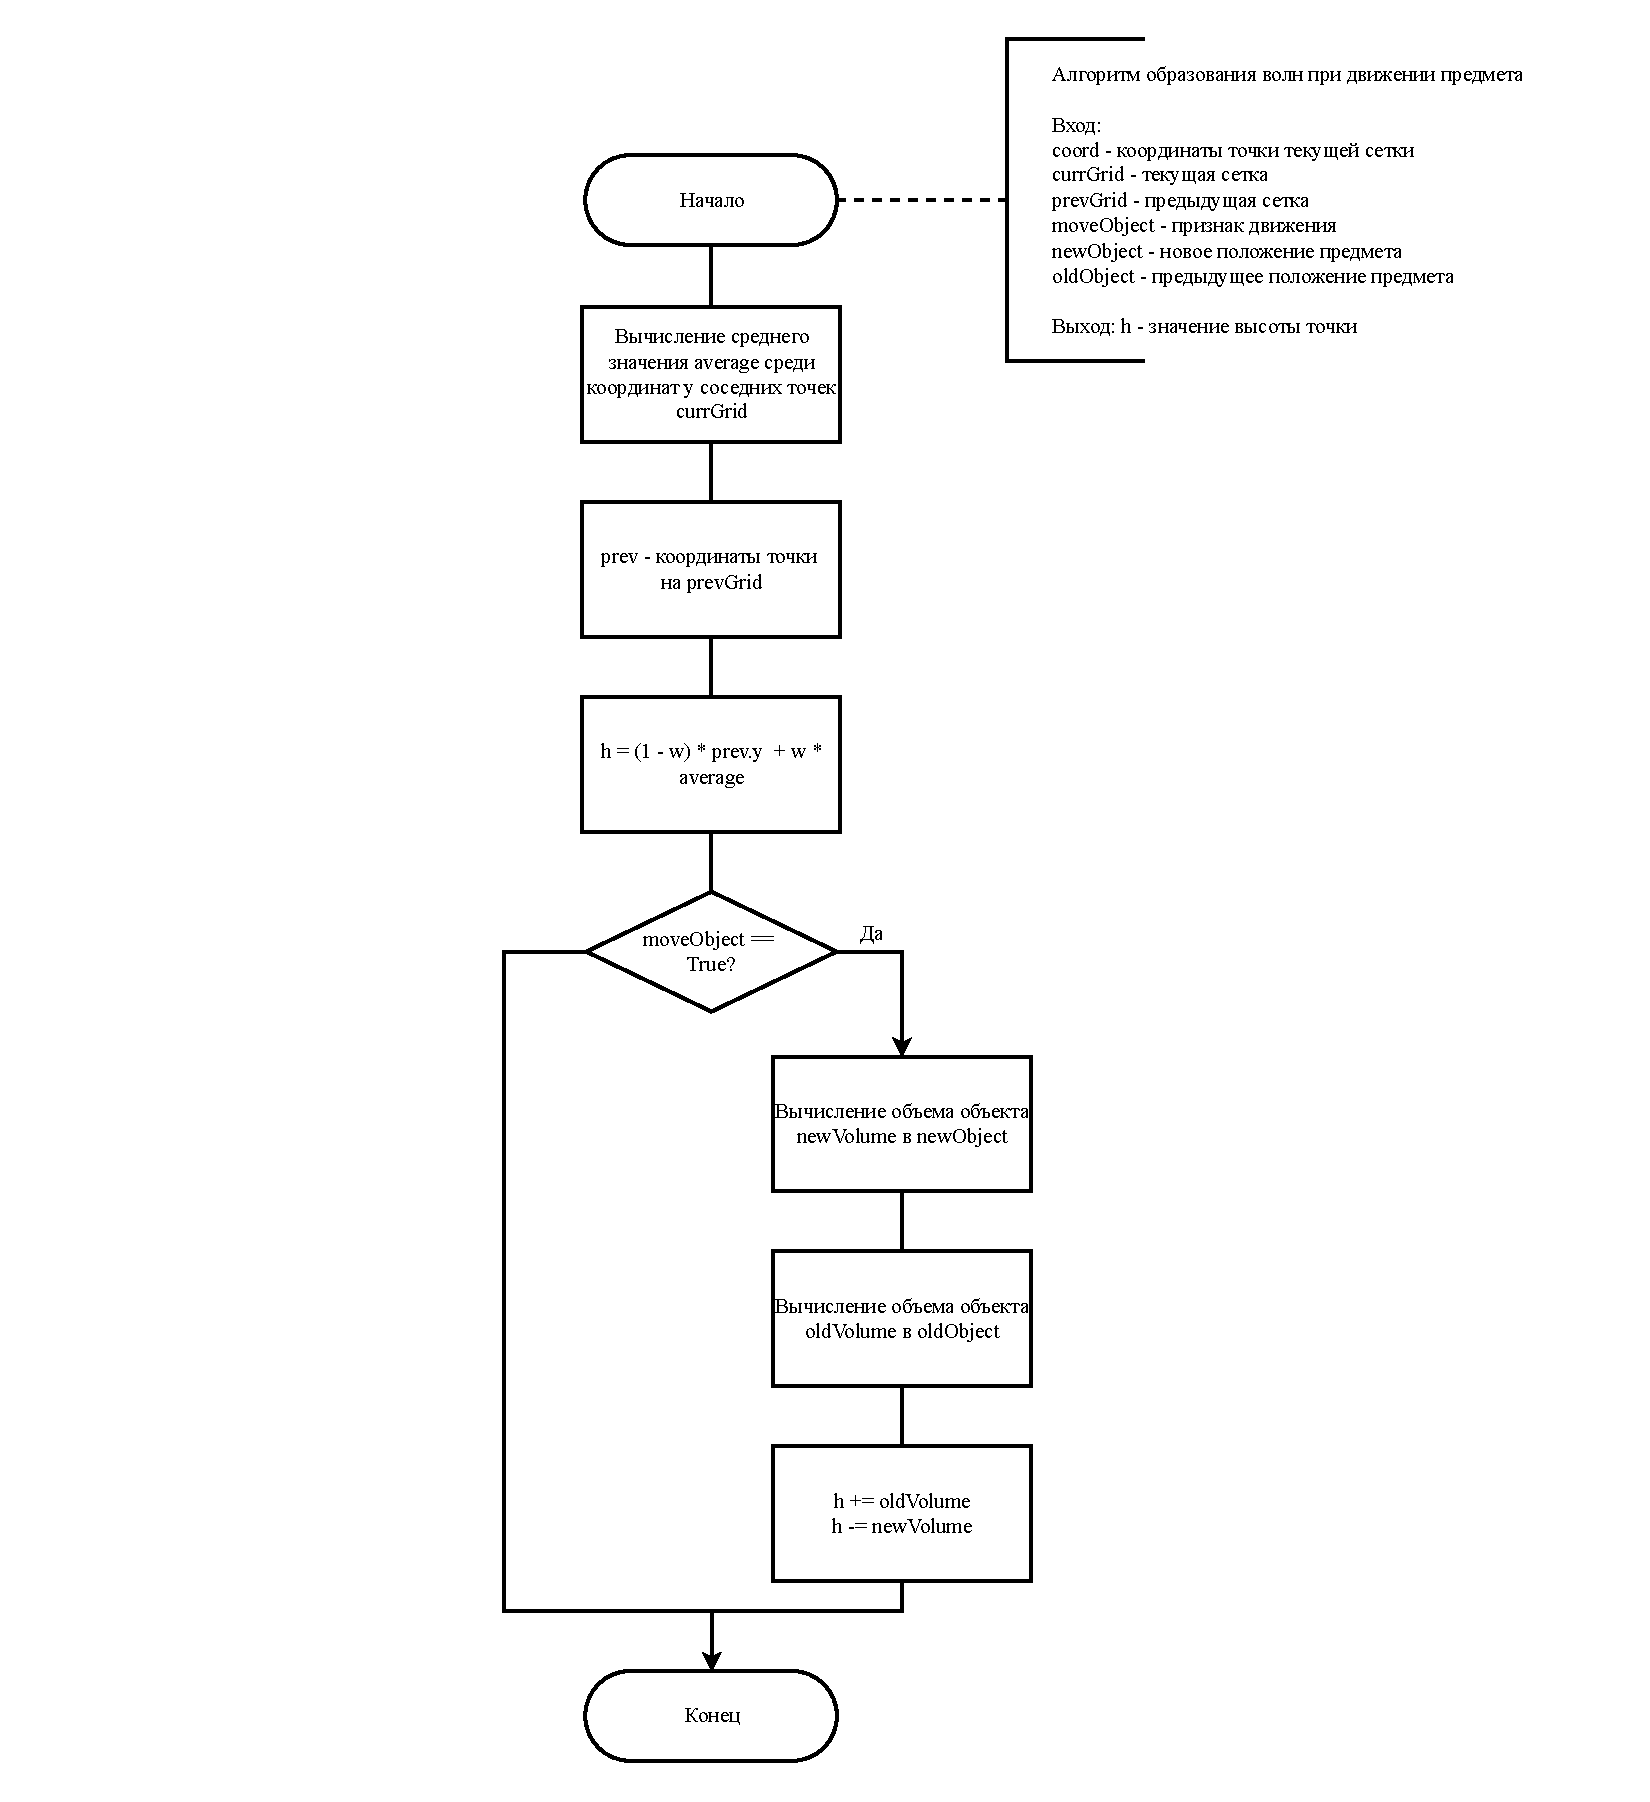
\includegraphics[scale=0.6]{img/alg-wave.pdf}
	\end{center}
	\captionsetup{justification=centering}
	\caption{Схема алгоритма образования волн при движении предмета}
	\label{img:alg-wave}
\end{figure}

\begin{figure}[H]
	\begin{center}
		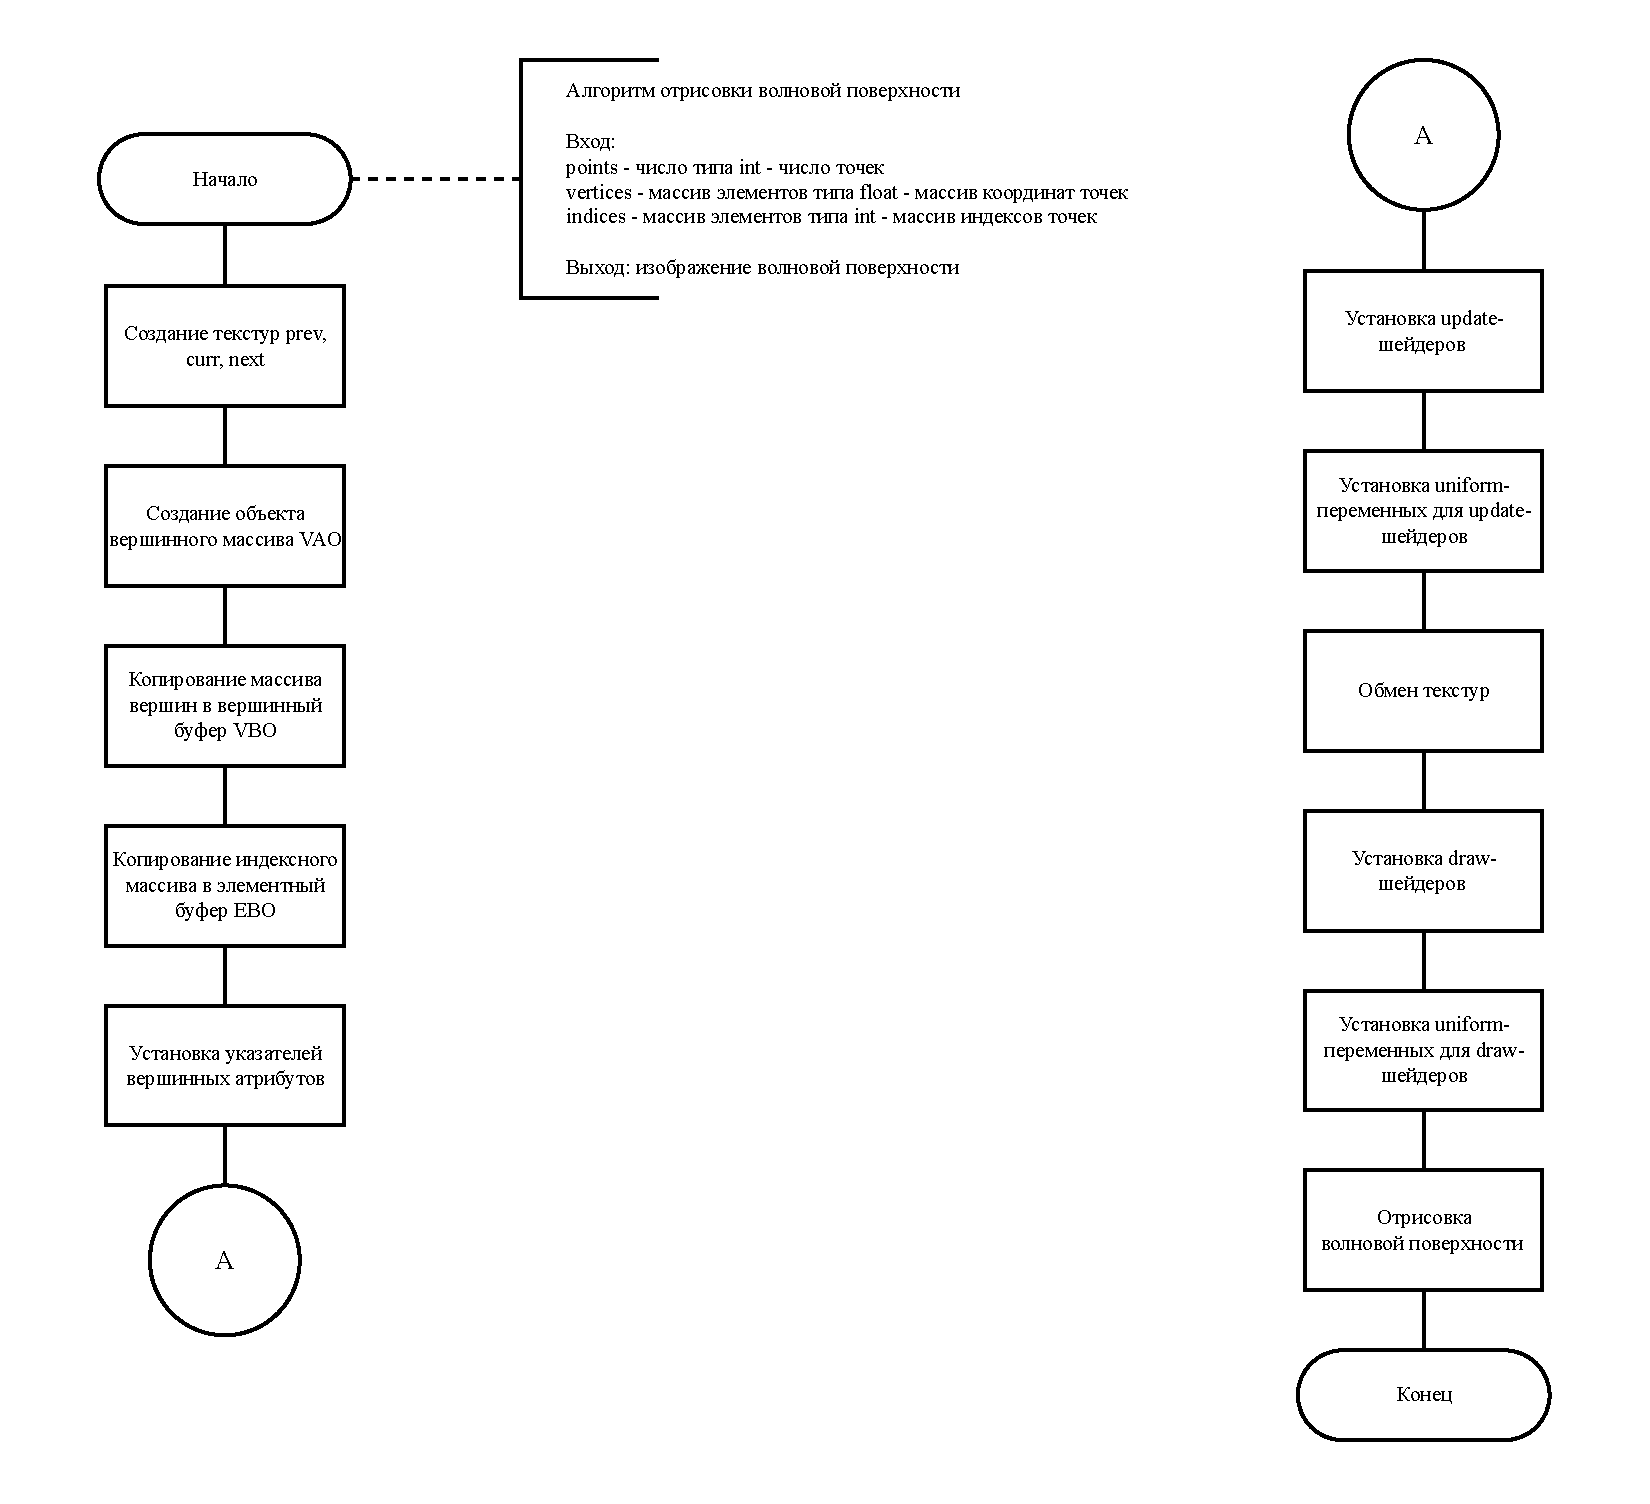
\includegraphics[scale=0.6]{img/draw-water.pdf}
	\end{center}
	\captionsetup{justification=centering}
	\caption{Схема алгоритма отрисовки волновой поверхности}
	\label{img:draw-water}
\end{figure}

\begin{figure}[H]
	\begin{center}
		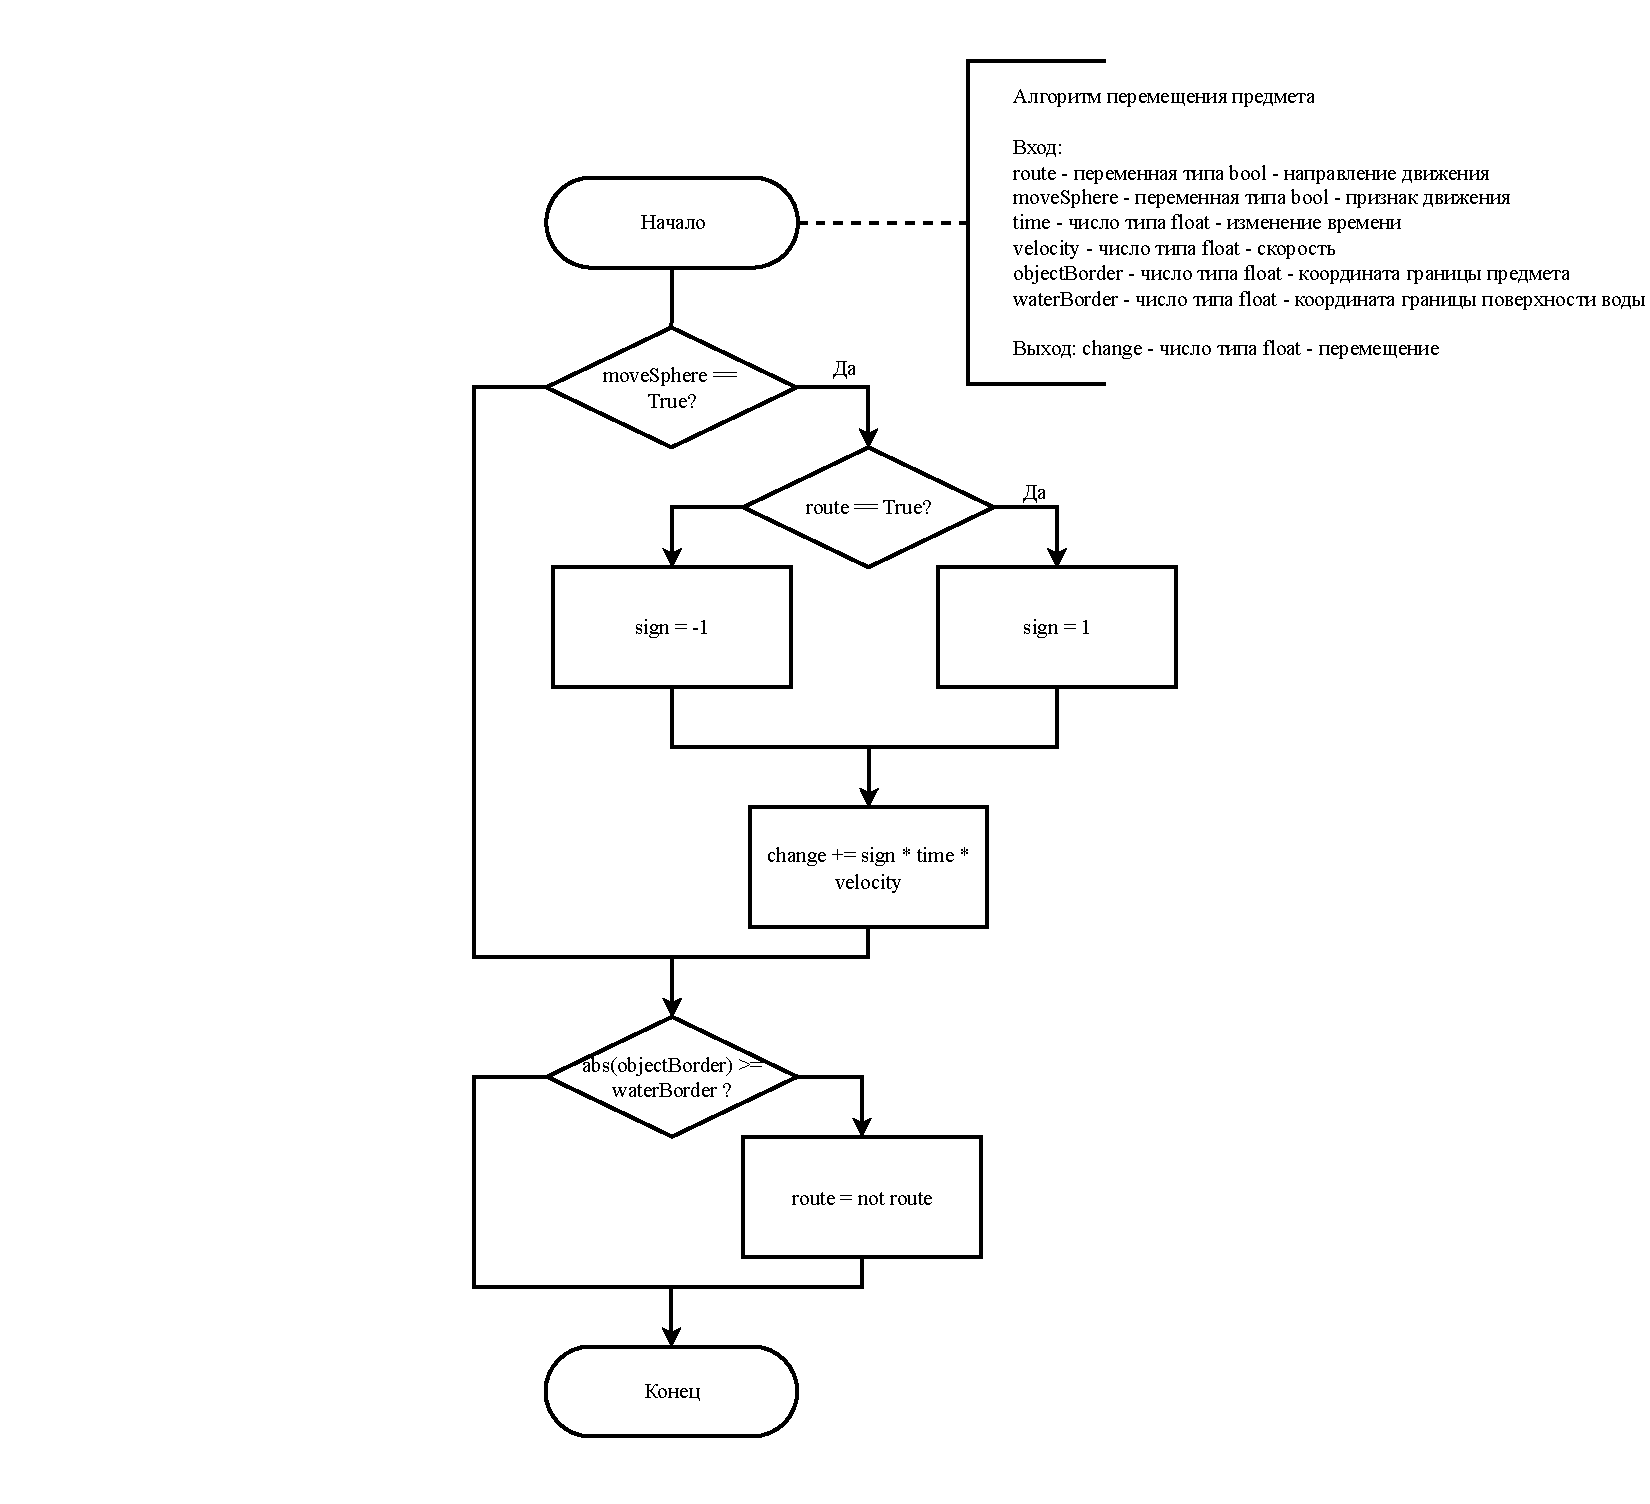
\includegraphics[scale=0.6]{img/move-object.pdf}
	\end{center}
	\captionsetup{justification=centering}
	\caption{Схема алгоритма перемещения предмета}
	\label{img:move-object}
\end{figure}

\begin{figure}[H]
	\begin{center}
		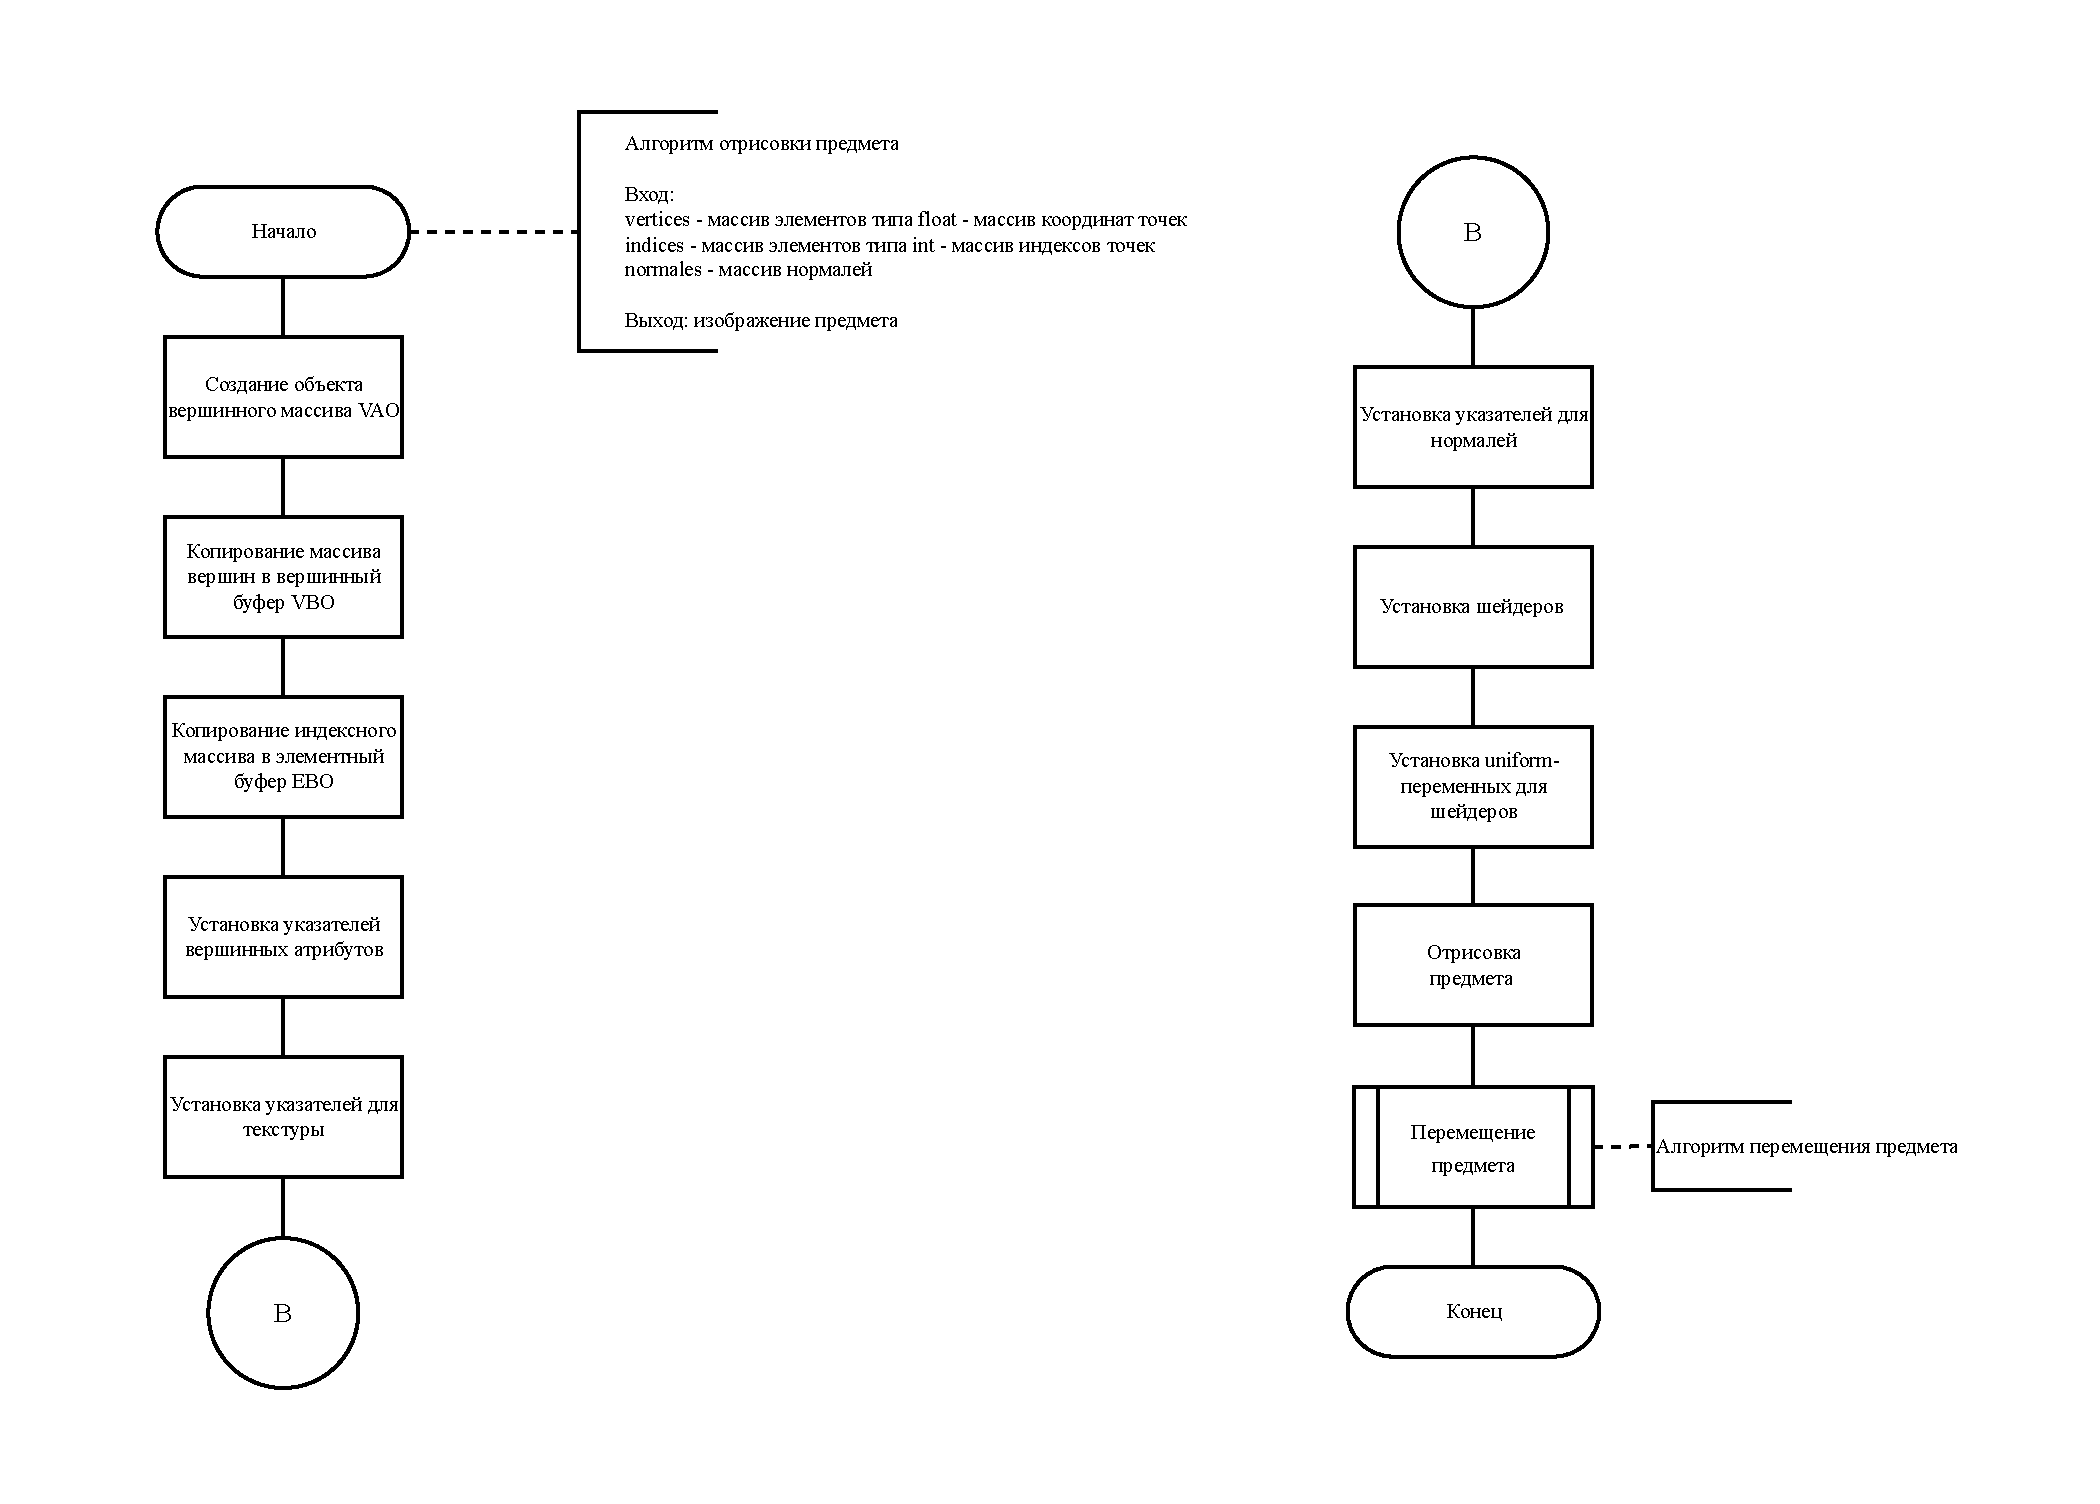
\includegraphics[scale=0.5]{img/draw-object.pdf}
	\end{center}
	\captionsetup{justification=centering}
	\caption{Схема алгоритма отрисовки предмета}
	\label{img:draw-object}
\end{figure}

\section{Описание используемых типов и \newline структур данных}

Для реализации поверхности воды используются следующие типы и структуры данных: 

\begin{itemize}
	\item для координат точек сетки --- трехмерный массив элементов типа float;
	\item для индексов точек сетки --- трехмерный массив элементов типа int;
	\item для числа точек сетки --- тип данных int.
\end{itemize}

Для создания предмета используются следующие типы и структуры данных:

\begin{itemize}
	\item для координат точек предмета --- трехмерный массив элементов типа float;
	\item для индексов точек предмета --- трехмерный массив элементов типа int.
\end{itemize}

Скорость движения задается числом типа int.

\section{Структура программного обеспечения}

На рисунке \ref{img:software-struct} представлена структура классов, реализованных в программном обеспечении.

\begin{figure}[H]
	\begin{center}
		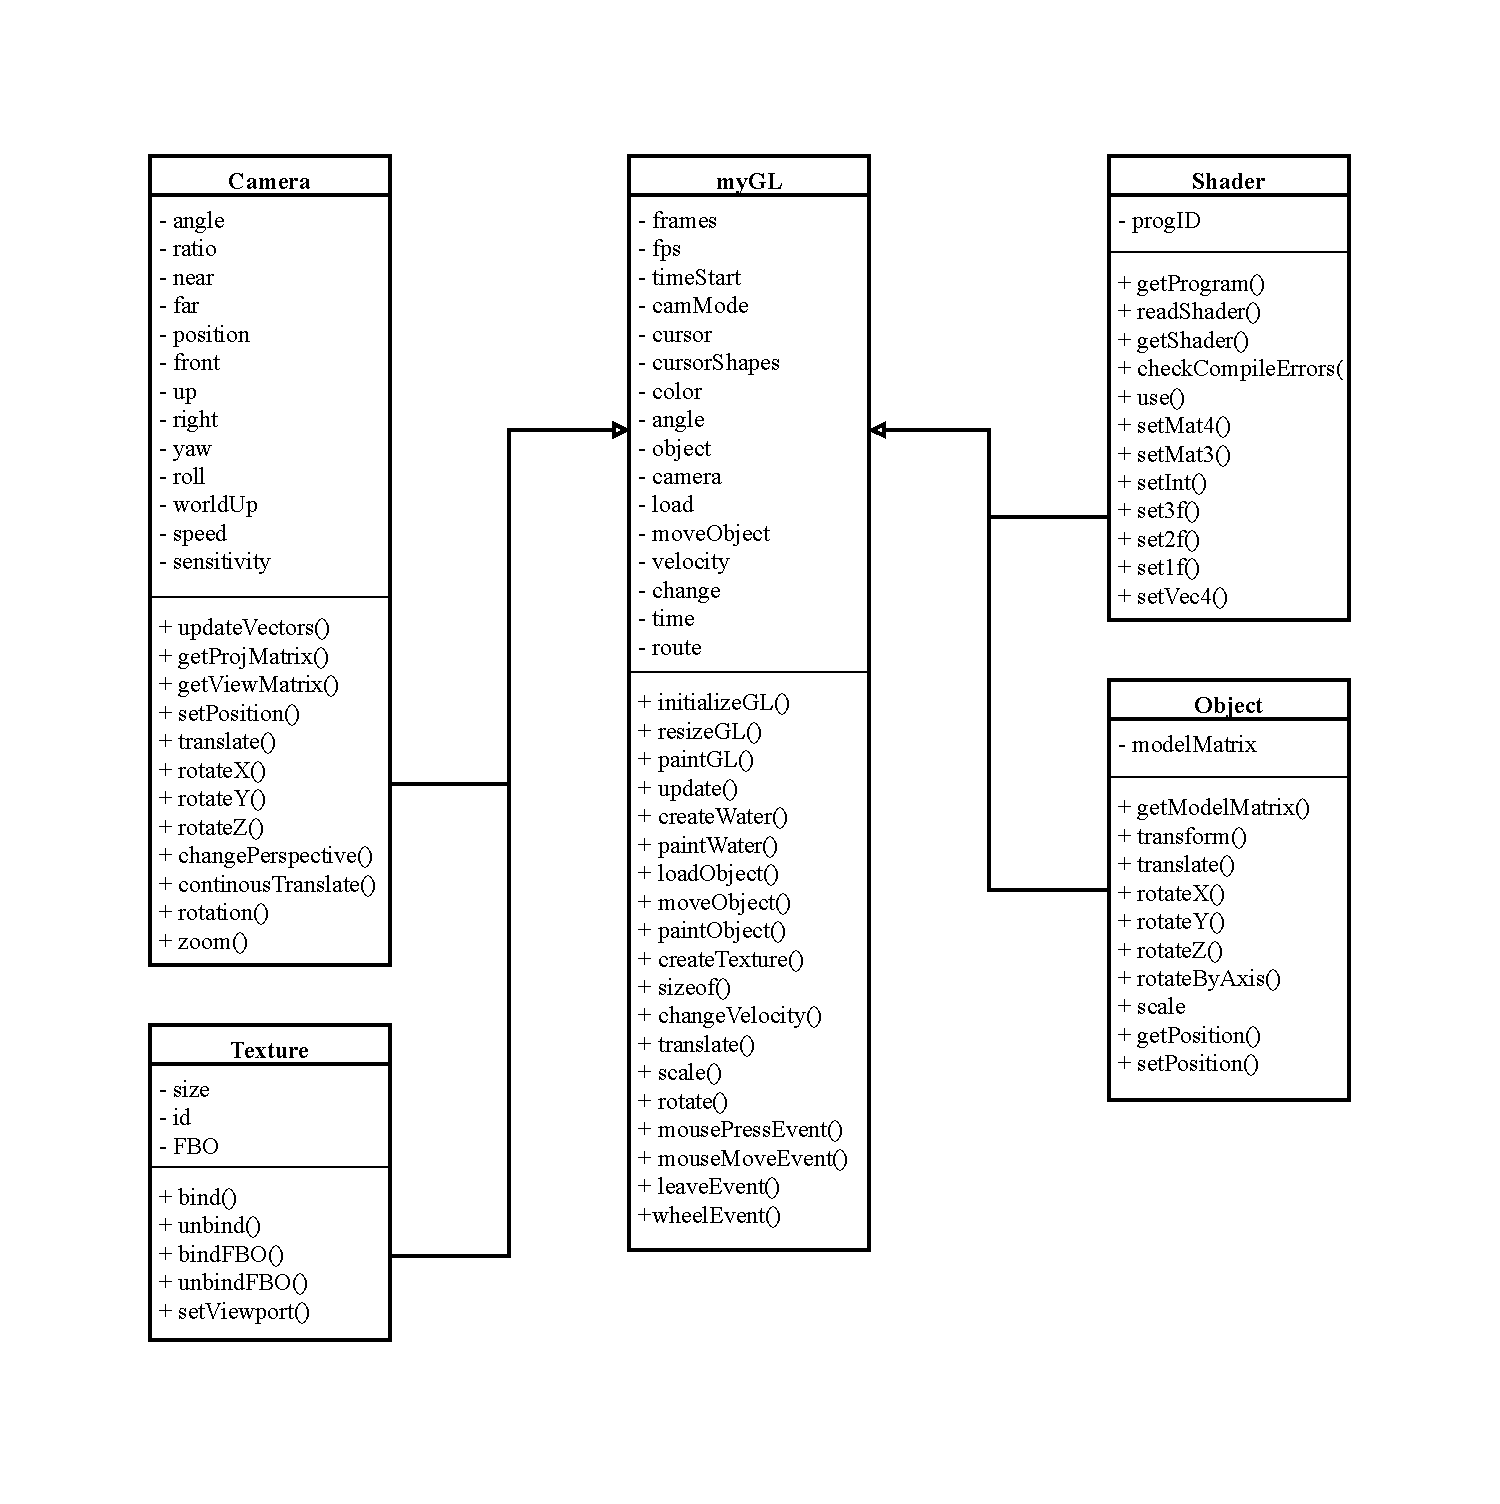
\includegraphics[scale=0.6]{img/software-struct.pdf}
	\end{center}
	\captionsetup{justification=centering}
	\caption{Структура реализуемых классов}
	\label{img:software-struct}
\end{figure}

Описание реализуемых классов:

\begin{itemize}
	\item myGL --- класс, в котором происходит отрисовка всех объектов сцены;
	\item Camera --- класс, предоставляющий функции работы с камерой;
	\item Texture --- класс для работы с текстурой и фрагментным буфером;
	\item Shader --- класс для загрузки шейдеров и установки uniform-переменных;
	\item Object --- класс, предоставляющий функции преобразования объектов сцены.
\end{itemize}

\section*{Вывод}

Были выделены требования к программному продукту, рассмотрены схемы алгоритмов моделирования и типы и структуры данных, при помощи которых реализуются методы визуализации, показана структура программного обеспечения.